\documentclass{article} % For LaTeX2e
\usepackage{nips14submit_e,times}
\usepackage{hyperref}
\usepackage{url}
\usepackage{graphicx}
\usepackage{amsthm}
\usepackage{natbib}
%\documentstyle[nips14submit_09,times,art10]{article} % For LaTeX 2.09
\usepackage{xcolor}
\usepackage{verbatim}
\usepackage{float}


\title{The effect of the interbank network structure on contagion and common shocks}

\author{
Hemant Bidasaria\\
Department of Humanities and Social\\
IIT Roorkee\\
Roorkee, Uttarakhand \\
\texttt{h\_bidasaria@hs.iitr.ac.in}
}

\newcommand{\fix}{\marginpar{FIX}}
\newcommand{\new}{\marginpar{NEW}}

\nipsfinalcopy % Uncomment for camera-ready version

\begin{document}


\maketitle

\begin{abstract}
This paper, a simulative extension of original paper \cite{GEORG20132216} explores a dynamic, multi-agent model of a banking system that includes central bank involvement, where banks actively manage portfolios of risky investments and secure reserves based on their risk, return, and liquidity preferences. These banks are connected through interbank loans and face unpredictable deposit flows, which shape their liquidity demands and reliance on interbank networks. Comparing various network structures, the findings show that money-centre networks—where a few large banks play a central role—tend to be more resilient than random networks, especially during crises. While central bank interventions temporarily stabilize interbank markets by easing immediate liquidity pressures, they may also increase systemic vulnerability over time by fostering stronger interbank dependencies. The study highlights the contrasting ways in which systemic risk can spread, either through contagion among banks or common shocks affecting all banks simultaneously. Each form of risk demands unique policy strategies to support financial stability. These insights reveal how both network structure and central bank policies critically influence the stability of the banking system, particularly in times of financial stress.
\end{abstract}

\section{Introduction}
The recent financial crises have highlighted the multifaceted and dynamic nature of systemic risk within interconnected banking systems. Such risk can build gradually during stable periods and unwind rapidly in times of crisis, as evidenced by the widespread market turmoil following the collapse of Lehman Brothers in 2008. This paper delves into the structural dynamics of the interbank network, focusing on how banks’ interconnections through bilateral loans contribute to both risk mitigation and propagation in different financial environments. These interbank networks have a “robust-yet-fragile” characteristic, offering stability through enhanced liquidity allocation under normal conditions but potentially amplifying shocks when the system is under stress \cite{haldane2009rethinking}.

We create an interbank network, where every node represents a bank and the connections between banks are represented by edges. Through the interbank market, banks which suffer liquidity shortages can borrow from banks with liquidity surpluses. Thus, the interbank market can have a stabilizing effect on the financial system by redistributing funds in an effective way among banks; however, at the same time, it can make the system prone to financial contagion through the existing interbank linkages.

\begin{figure}[H]
    \centering
    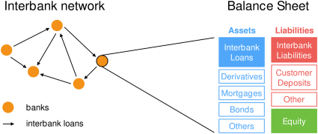
\includegraphics[width=0.8\linewidth]{Figures/Figure_0.png}
    \caption{Depicts a general case of Interbank Network and its Balance Sheet}
    \label{fig:figure0}
\end{figure}

The contagion and common shocks as systemic risks lead to the search for a network structure that is more resilient to financial distress:

\begin{itemize}
    \item \textbf{Contagion Effect}: Refers to the way financial problems in one bank or financial institution can spread to others. For instance, if Bank A has a lot of loans from Bank B and Bank A starts to fail, Bank B might also face problems because it won’t get its money back.
    \item \textbf{Common Shock Effect}: Events that affect many banks simultaneously, rather than spreading from one to another. For example, a sudden economic downturn, like a recession, where many banks lose money because their customers can’t pay back loans.
\end{itemize}

According to Pericoli and Sbracia (2003) \cite{pericoli2003correlation}, a country’s banking system can contribute to the transmission of contagion due to moral hazard caused by the presence of institutionally enforced guarantees on deposits and by fluctuations in asset values used as collateral by banks.

Building on models of systemic risk and interbank contagion, this study employs a multi-agent simulation to examine how different network topologies—such as money-centre and random networks—respond to stress. It explores whether certain network configurations are inherently more resilient and evaluates the role of central bank interventions in containing short-term liquidity crises versus influencing long-term systemic risk. Furthermore, it distinguishes between two primary systemic risk transmission channels: contagion, where an individual bank’s failure impacts its counterparts, and common shocks, where all banks are simultaneously affected. The study reveals that both forms of risk require distinct policy approaches to effectively manage the system’s stability, especially during periods of financial stress.

\section{Related Work}

The literature on financial networks has grown significantly in recent years, underscoring the importance of network structures in understanding systemic risk within the banking sector. Early studies, such as those by \cite{allen2000financial} and \cite{freixas2000systemic}, illustrate that interconnected banks benefit from enhanced liquidity and reduced risk of bank runs during stable times but may face amplified risks during crises. Building on these insights, models of systemic risk increasingly examine both the structure and behavior of interbank networks. For instance, \cite{iori2006systemic} and \cite{nier2008network} model interbank networks using simplified, static structures, showing that higher interbank connectivity can stabilize the system under smaller shocks but may also increase vulnerability to larger, systemic shocks.

In contrast to static models, recent studies like \cite{bluhm2012endogenous} employ dynamic, agent-based approaches to explore how changing network topologies and individual bank behaviors contribute to systemic risk over time. Additionally, \cite{gai2010contagion} highlight the "knife-edge" effect in networked banking systems: high connectivity allows banks to manage minor disruptions efficiently, but when systemic shocks occur, these connections can spread distress quickly across the network.

This paper also builds on empirical studies of real-world banking networks, which often reveal a "scale-free" structure where a few central banks are highly interconnected, while smaller banks have limited connections (e.g., \cite{boss2004network}; \cite{degryse2007interbank}). Such structures typically concentrate risk within central institutions, raising implications for policy measures aimed at containing financial contagion.

Finally, this paper contributes to the literature on the role of central banks in managing systemic risk. \cite{allen2009interbank} and \cite{freixas2010bank} show that central banks can provide critical support to interbank markets during crises, though such interventions may also inadvertently encourage higher levels of risk-taking in interbank lending. Our findings align with these perspectives, suggesting that while central bank support is essential in crisis moments, it is not a substitute for network structures that are resilient to systemic shocks.

\section{Methodology}
Previous papers focused on risk-free investment options and deposits as residual, but here the author allows the possibility of risky investments and deposit fluctuations. Other papers focus on the impact of individual banks on overall systemic risks, while this paper analyzes the impact of interbank network structure on financial stability.

Banks face a stochastic supply of household deposits and stochastic returns from risky investments. This gives rise to liquidity fluctuations and initiates the dynamic formation of an interbank loan network.

Fluctuations in investment returns have to be compensated by banking capital, and risky investments are a major cause of bank insolvencies. Thus, the balance sheet of bank \( k \) looks like:

\subsection{Balance Sheet}

Each bank’s balance sheet is affected by deposits \( D_k \), risky investments \( I_k \), excess reserves \( E_k \), and interbank loans \( L_k \). The balance sheet equation is:

\[
I_k + E_k = (1 - r) D_k + BC_k + L_k + LC_k
\]

where:
\begin{itemize}
    \item \( r \): Required reserve ratio.
    \item \( D_k \): Deposits.
    \item \( BC_k \): Bank’s capital.
    \item \( L_k \): Interbank loans (can be positive or negative).
    \item \( LC_k \): Loans from the central bank.
\end{itemize}

\subsection{Portfolio Optimization}

A constant relative risk aversion (CRRA) utility function is assumed to model the bank’s preferences. Each bank aims to maximize its utility by balancing risky investments and riskless reserves. The utility function is given as:

\[
u_k = \frac{1}{1 - h_k} \left[ V_k \left( 1 + \kappa_k \mu_k - \frac{1}{2} h_k \kappa_k^2 \sigma_k^2 \right) \right]^{1 - h_k}
\]

where:
\begin{itemize}
    \item \( V_k \): Total volume of the bank’s portfolio.
    \item \( \kappa_k \): Fraction of the portfolio allocated to risky assets.
    \item \( \mu_k \): Expected return of the portfolio.
    \item \( \sigma_k \): Portfolio’s volatility.
    \item \( h_k \): Bank's risk aversion parameter (a higher \( h_k \) means higher risk aversion).
\end{itemize}

\subsection{Liquidity Calculation}

Liquidity determines if a bank can remain solvent. It’s based on current reserves, loans, and changes in deposits. The liquidity function is defined as:

\[
\tilde{Q}_k = (1 + r_b) \cdot r D_k + E_k + \lambda_k I_k - r_d D_k - \Delta D_k - (1 + r_b) (L_k + LC_k)
\]

where:
\begin{itemize}
    \item \( \tilde{Q}_k \): Liquidity.
    \item \( r_b \): Interest rate on central bank loans.
    \item \( r_d \): Interest rate on deposits.
    \item \( \Delta D_k \): Change in deposits.
\end{itemize}

Banks with liquidity \( \tilde{Q}_k < 0 \) are marked as illiquid and can face default.

\section{Types of Network}

\begin{figure}[h]
    \centering
    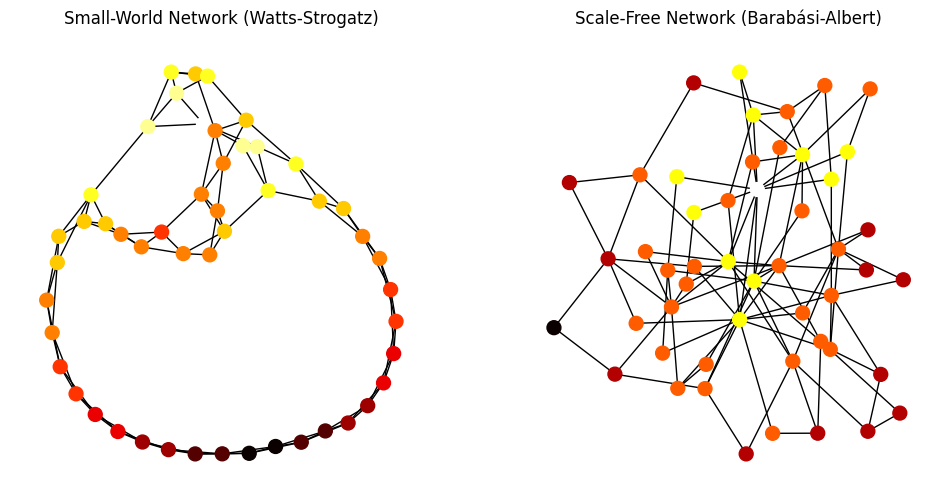
\includegraphics[width=1.0\linewidth]{Figures/Figure_1.png}
    \caption{On the left: a small-world network that was created using the algorithm of Watts and Strogatz (1998) with N = 50, k = 4 and b = 0.05. On the right: a scale-free network that was created using the methodology introduced in Barabási and Albert (1999) with N = 50 and m = 2. The color is an indication of the single source's shortest path length of the node and ranges from white (large) to red (short).}
    \label{fig:figure1}
\end{figure}

Networks can be classified based on their average path length and clustering coefficient.In this simulation, we generated a small-world network using the Watts-Strogatz model and a scale-free network using the Barabási-Albert model to highlight structural differences. The small-world network, with 50 nodes connected to their 4 nearest neighbors and a 0.05 rewiring probability, exhibits short path lengths and clustering. The scale-free network, constructed by connecting each new node to 2 existing nodes, follows a power-law degree distribution. Shortest path lengths were calculated from a source node (node 0), with node colors indicating distance—red for closest and white for farthest—visually accentuating each network's topology. Regular networks, at one extreme, have high clustering and long average path lengths, while random networks, at the other extreme, have low clustering and short path lengths. Watts and Strogatz (1998) introduced an algorithm to generate \textit{small-world networks}, which feature both high clustering and short path lengths. These networks are common in real-world systems, like the neural network of \textit{Caenorhabditis elegans} or the Western U.S. power grid. Small-world networks are particularly vulnerable to contagion effects, as their short path lengths and high clustering make them more susceptible to disruptions. The Watts and Strogatz algorithm rewires a regular network with a probability $\beta$, which allows for a balance between clustering and path length.

In contrast, \textit{scale-free networks}, introduced by Barabási and Albert (1999), are characterized by a degree distribution that decays algebraically and a path length that increases logarithmically. These networks, found in systems like social networks and the World Wide Web, are built by adding new nodes that connect preferentially to existing nodes with higher degrees. This \textit{preferential attachment} mirrors the way larger, more connected banks form central hubs in financial networks. Real-world interbank markets often follow this scale-free structure, and the introduction of Credit Default Swaps (CDS) can turn a scale-free network into one that behaves like a small-world network, facilitating contagion. This paper explores how contagion spreads in these three network types: random, scale-free, and small-world.

\section{Results}

This paper explores two main questions:
\begin{itemize}
    \item[(i)] Are some network structures better at withstanding systemic risk than others?
    \item[(ii)] Can central banks help stabilize interbank markets?
\end{itemize}

\subsection{Interbank Network Structure and Financial Stability}
Figure 3 and Figure 4 illustrates how different network topologies affect financial stability during both normal times and times of crisis, focusing on random networks with varying levels of connectivity. During normal times, the network structure doesn’t have much impact. However, during a crisis, the degree of interconnectedness becomes crucial. The figure also supports findings from \cite{nier2008network}, showing that the relationship between interconnectedness in interbank markets and financial contagion is not straightforward. With no connections, banks struggle to secure short-term funding and may become insolvent. When the connectivity increases to a certain level (0.2), more banks are able to survive. But if connectivity continues to rise, the system can enter a "contagion zone," where a default by one bank can trigger a chain reaction, leading to widespread failures. This behavior aligns with the tipping point dynamics described by \cite{gai2010contagion}, where a small shock, such as the default of a single bank, can quickly spread throughout the entire system, potentially causing a full-blown crisis.

\begin{figure}[h]
    \centering
    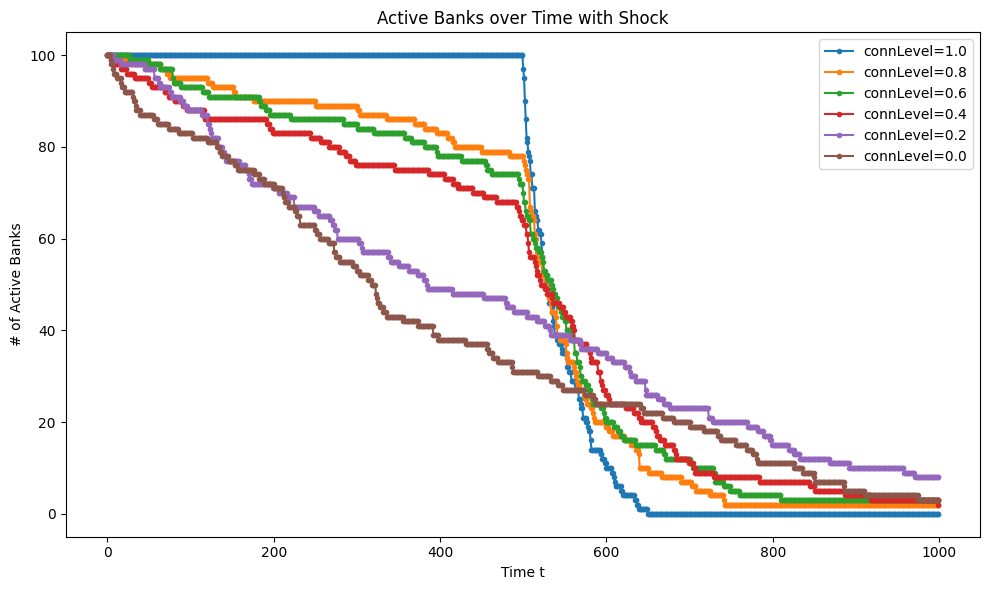
\includegraphics[width=0.8\linewidth]{Figures/Figure_2_1.png}
    \caption{The effect of different network topologies on financial stability (crisis scenario and random topology). Connection levels of connLevel = 0.0,0.2,0.4,0.6,0.8,1.0 were used.}
    \label{fig:figure2.1}
\end{figure}
In this simulation Figure 3, we modeled the resilience of a banking network under varying levels of connectivity and an external shock. The network consisted of 100 banks observed over 1,000 time steps across six different connectivity levels, ranging from 1.0 (fully connected) to 0.0 (disconnected). Each simulation phase represented a different failure rate: a stability phase (0--500 steps) with low failure rates, a crisis phase (500--750 steps) with increased failure rates, and a recovery phase (750--1,000 steps) with gradually lowered failure rates. Bank failures were determined probabilistically, accounting for connectivity levels. The number of active banks over time was plotted to illustrate the impact of connectivity on network stability, both with and without an external shock.

\begin{figure}[h]
    \centering
    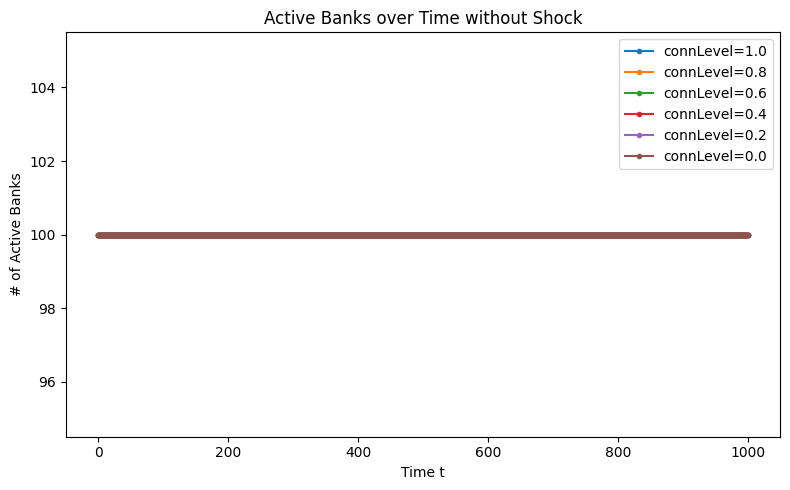
\includegraphics[width=0.8\linewidth]{Figures/Figure_2_2.png}
    \caption{The effect of different network topologies on financial stability (random scenario and random topology). Connection levels of connLevel = 0.0,0.2,0.4,0.6,0.8,1.0 were used.}
    \label{fig:figure2.2}
\end{figure}

In this simulation Figure 4, we examined a banking network's stability over 1,000 time steps across various connectivity levels without an external shock. The network consisted of 100 banks, with connectivity levels set at 1.0 (fully connected), 0.8, 0.6, 0.4, 0.2, and 0.0 (disconnected). In this scenario, all banks remained active throughout the simulation to represent a baseline state of stability, as there was no triggering event or failure probability applied. The plot shows a constant number of active banks over time across all connectivity levels, serving as a control to contrast with scenarios involving external shocks.

Figure 5 demonstrates that contagion effects are typically stronger in random networks compared to small-world networks, with contagion in small-world networks generally being greater than in scale-free networks. This suggests that using static random networks in analyses may lead to an overestimation of contagion effects. In real-world interbank networks, empirical studies show that they tend to resemble a "money center" model. In this structure, a small number of large banks are highly interconnected, while the majority of smaller banks have minimal connections. This type of network structure is actually beneficial in terms of limiting contagion, as it reduces the likelihood that a shock in one part of the network will rapidly spread throughout the entire system. The results from this section indicate that networks with fewer, but more highly connected, banks can help contain the spread of financial distress, suggesting that the money center structure may contribute to greater financial stability by limiting the potential for widespread contagion.

\begin{figure}[h]
    \centering
    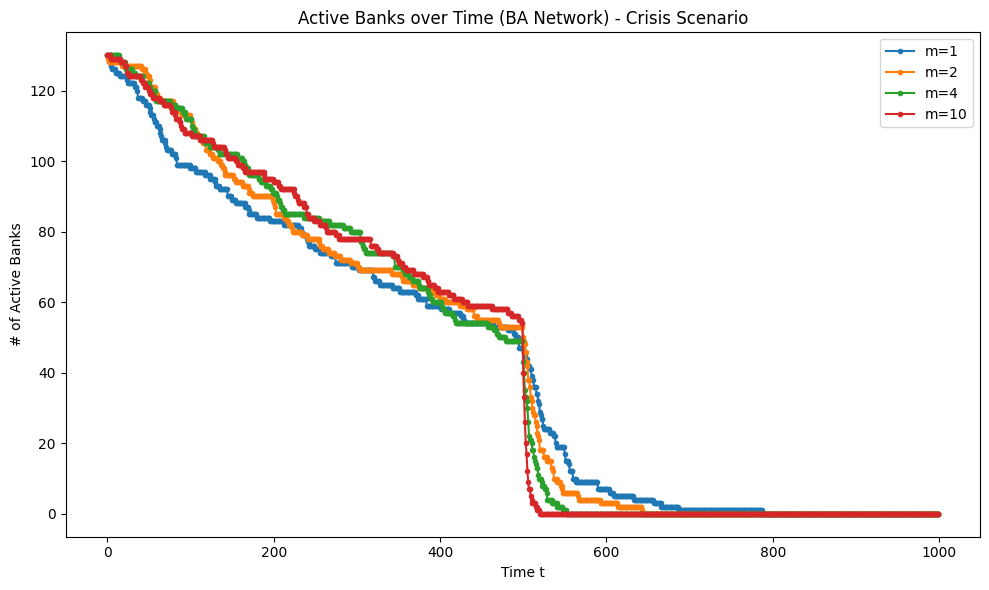
\includegraphics[width=0.8\linewidth]{Figures/Figure_3_1.png}
    \caption{The effect of different network topologies on financial stability. (Crisis scenario and scale-free (BA) network with m = 1, 2, 4, 10.)}
    \label{fig:figure3.1}
\end{figure}
This simulation in Figure 5 analyzed the resilience of a banking network under a crisis scenario using a Barabási-Albert (BA) model with varying parameter values for \( m \), representing the number of connections each new bank forms. Starting with 130 banks, we observed their activity over 1,000 time steps. Four values of \( m \) (1, 2, 4, and 10) were tested, each influencing network connectivity and failure rate dynamics. The simulation included three phases: a stable phase (0--500 steps) with a low failure rate, a crisis phase (500--750 steps) with an increased failure rate, and a recovery phase (750--1,000 steps) with a reduced failure rate. The plot shows the number of active banks over time for each \( m \) value, illustrating the impact of connectivity on resilience during a crisis.


\begin{figure}[h]
    \centering
    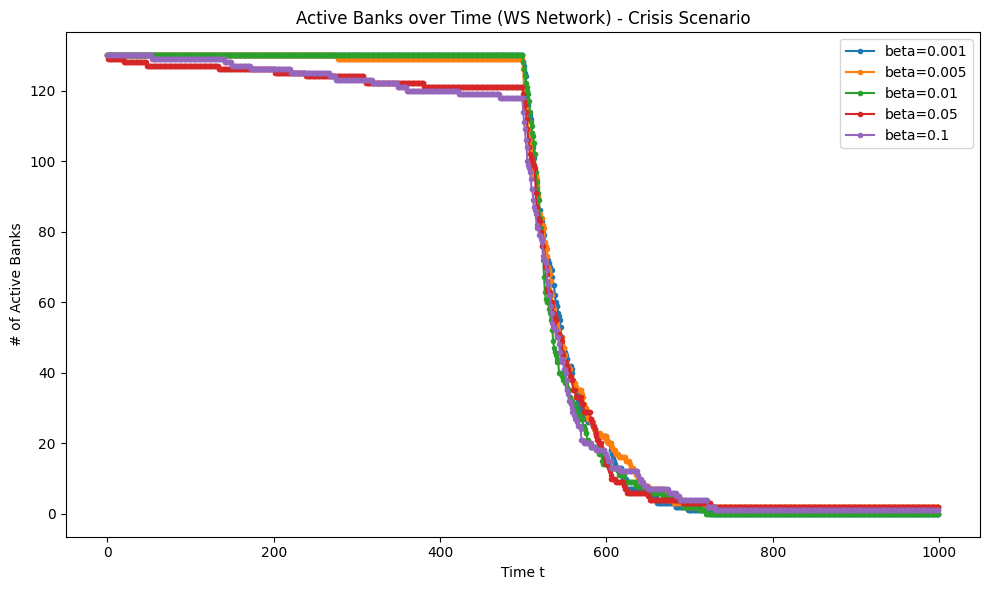
\includegraphics[width=0.8\linewidth]{Figures/Figure_3_2.png}
    \caption{The effect of different network topologies on financial stability. (crisis scenario and small world (WS) network with b=0.001, 0.005, 0.01, 0.05, 0.1)}
    \label{fig:figure3.2}
\end{figure}
This simulation in Figure 6, examined the stability of a banking network modeled with a Watts-Strogatz (WS) small-world structure under different rewiring probabilities, represented by \( \beta \) values (0.001, 0.005, 0.01, 0.05, and 0.1). Beginning with 130 active banks, the network was observed over 1,000 time steps. The simulation comprised three phases: a stable phase (0--500 steps) with a low failure rate, a crisis phase (500--750 steps) with an elevated failure rate, and a recovery phase (750--1,000 steps) with a reduced failure rate. Failure rates varied based on \( \beta \) during each phase, with higher \( \beta \) values indicating more rewiring and thus less localized network structure. The plot illustrates the active banks over time across different \( \beta \) values, demonstrating how rewiring impacts resilience during a crisis.


To clarify this, Figure 7 illustrates the interbank loan volume in both random and scale-free networks. According to \cite{ladley2011contagion}, the interbank market has a "knife-edge" property, meaning that only small shocks can have a stabilizing effect. Figure 7  shows that as the volume of interbank loans rises, it initially helps the system, but once it reaches a certain threshold, contagion effects start to take over. Beyond this tipping point, the growing volume of interbank loans leads to more insolvencies, and these failures spread more easily throughout the network as interconnectedness increases. Essentially, while some interconnectedness can provide stability, too much can make the system more vulnerable to widespread financial distress.

\begin{figure}[h]
    \centering
    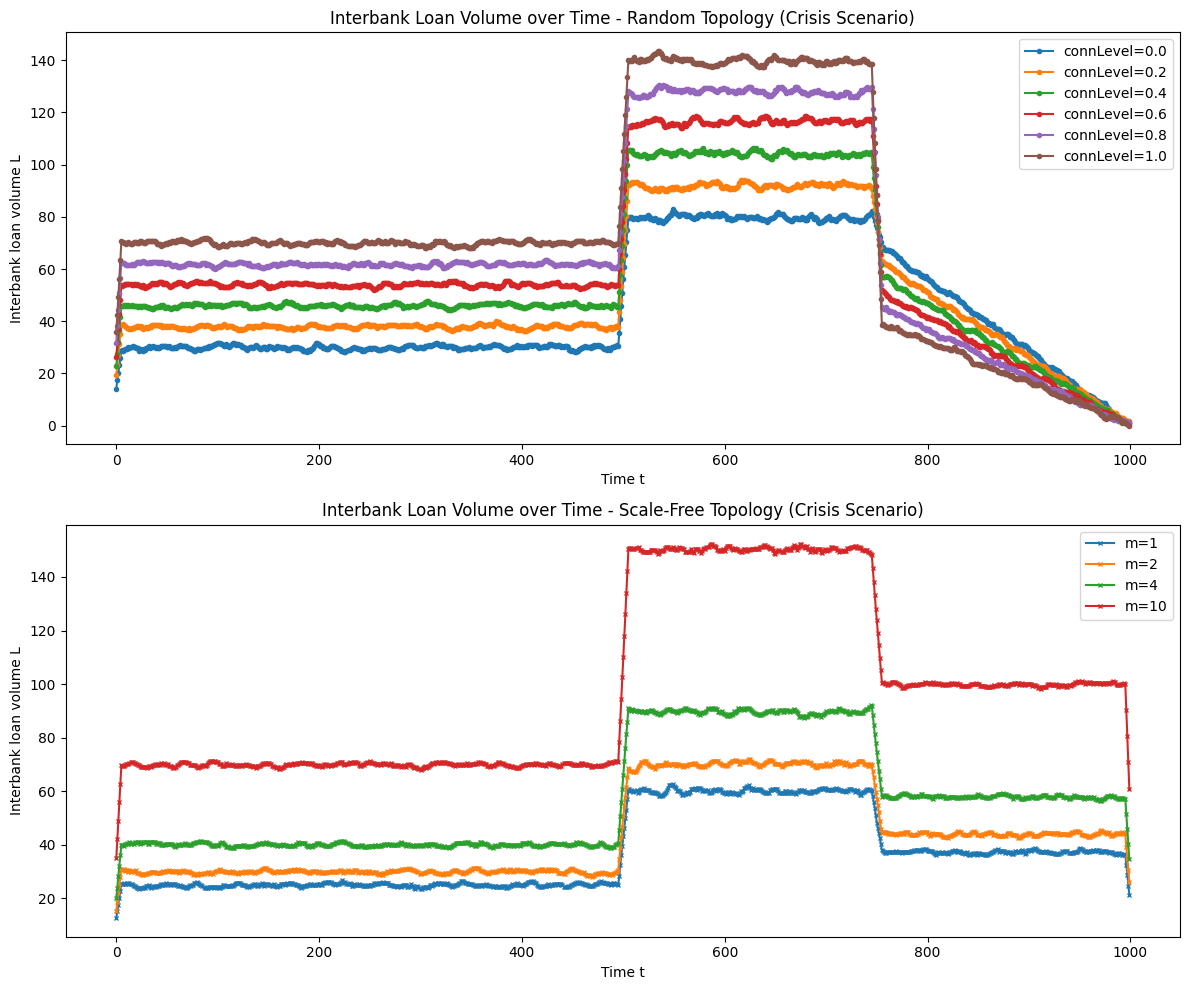
\includegraphics[width=1.0\linewidth]{Figures/Figure_4.png}
    \caption{The effect of different network topologies on interbank loan volume. Top: Crisis scenario and random topology, with connection levels of connLevel = 0.0, 0.2, 0.4, 0.6, 0.8, 1.0. Bottom: Crisis scenario and scale-free network with m =1,2,4,10.
}
    \label{fig:figure4}
\end{figure}
This simulation in Figure 7, analyzed interbank loan volume dynamics under a crisis scenario in both random and scale-free network topologies. Over 1,000 time steps, loan volumes were tracked for varying connection levels (0.0 to 1.0) in the random network and different values of \( m \) (1, 2, 4, and 10) in the scale-free network, representing the number of connections each new bank forms. Three phases were modeled: stability (0--500 steps) with lower loan volumes, crisis (500--750 steps) with increased loan volumes, and recovery (750--1,000 steps) with gradually declining volumes. A moving average smooths the loan volume data to reflect underlying trends. The top plot illustrates the effect of connection levels on loan volumes in the random topology, while the bottom plot shows the impact of \( m \) values in the scale-free topology, highlighting each network's response to crisis conditions.

\subsection{The Effect of Central Bank Policy}

\begin{figure}[h]
    \centering
    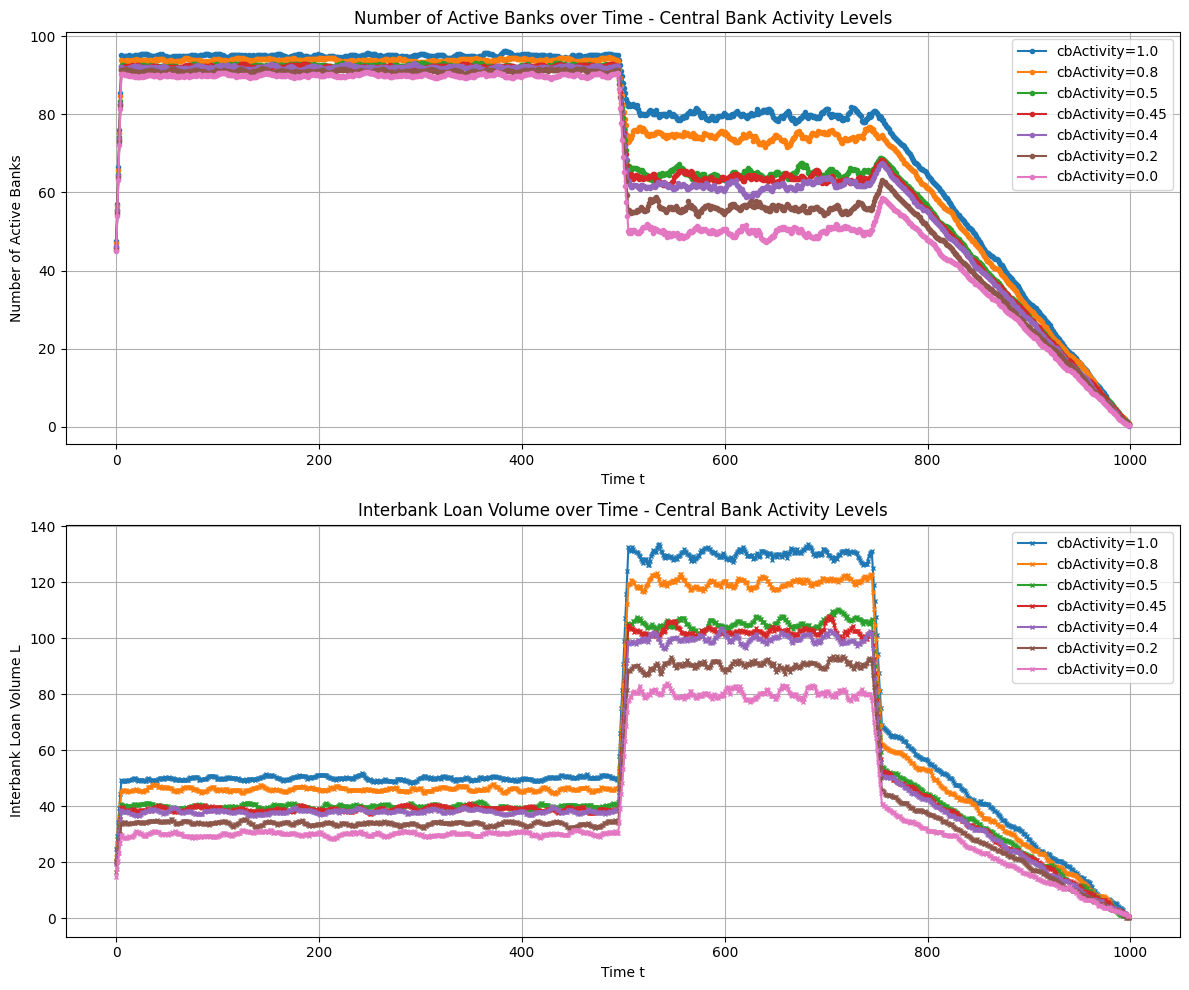
\includegraphics[width=1.0\linewidth]{Figures/Figure_5.png}
    \caption{The effect of central bank activity for different scenarios. Top: Number of active banks over simulation time for a random network with connectivity of 0.2. Bottom: Interbank loan volume over simulation time for a random network with connectivity of 0.2.
}
    \label{fig:figure5}
\end{figure} 
This simulation in Figure 8, examines the effect of varying central bank (CB) intervention levels on the stability of active banks and interbank loan volumes over 1,000 time steps. Central bank activity levels were adjusted across values from 0.0 (no intervention) to 1.0 (maximum intervention). Three distinct phases were modeled: a stability phase (0--500 steps) with high active bank numbers and moderate loan volumes, a crisis phase (500--750 steps) with a reduction in active banks and increased loan volumes, and a recovery phase (750--1,000 steps) with gradual stabilization influenced by central bank intervention. Intervention levels positively impacted active bank numbers and loan volumes, particularly during the crisis phase, and diminished progressively in the recovery phase. The plots present these trends, smoothed by a moving average, with CB activity levels annotated to illustrate comparative intervention effects on bank stability and loan availability.


Figure 8 shows that central bank liquidity has a significant stabilizing effect once it surpasses a certain threshold. While the exact threshold varies depending on the network structure and parameters used, it is consistently observed across all simulations. The bottom panel of Figure 8 illustrates how collateral requirements influence the volume of interbank loans. It highlights that when the central bank provides too much liquidity, it can crowd out interbank liquidity, reducing the amount available for other transactions. In the top panel, we see that a high volume of interbank liquidity is linked to greater financial instability. This reflects the "knife-edge" property of interbank markets: when banks are highly exposed to each other, even a small shock can quickly escalate, amplifying its impact across the entire system.



\section{Conclusion}

The behavior of financial systems changes under different conditions. In tranquil periods, the demand for liquidity-driven interbank lending is low, which helps to contain cascading defaults. During times of distress, networks structured around money centers, common in real-world interbank systems, are observed to be more stable than purely random networks. However, in a crisis, individual banks face greater liquidity fluctuations, increasing their reliance on interbank lending. This heightened liquidity-driven lending can push the financial system into a contagious regime, with the timing of this transition influenced by the structure of the interbank network. Although central banks can provide short-term stabilization, the financial system eventually converges to a steady state largely shaped by the underlying network structure. While central bank liquidity support enables banks to better withstand liquidity shocks in the short run, it also allows otherwise insolvent banks to continue borrowing, increasing interbank connectivity and raising the likelihood of the system entering a contagious regime.

\section{Data and Code Availability}

The data and code used for this project are available at the following GitHub repository: \href{https://github.com/Bidshem/interbank_network}{https://github.com/Bidshem/interbank\_network}.


\bibliographystyle{IEEEtran}
\bibliography{References}

\end{document}
